\section{Appendix Results}
\label{app:results_appendix}

\subsection{Batch 1 Stage-by-Stage Results}

\begin{figure}[!htbp]
    \centering
    \caption{Extensive Outcomes: Stage-by-Stage Effects, Batch 1}
    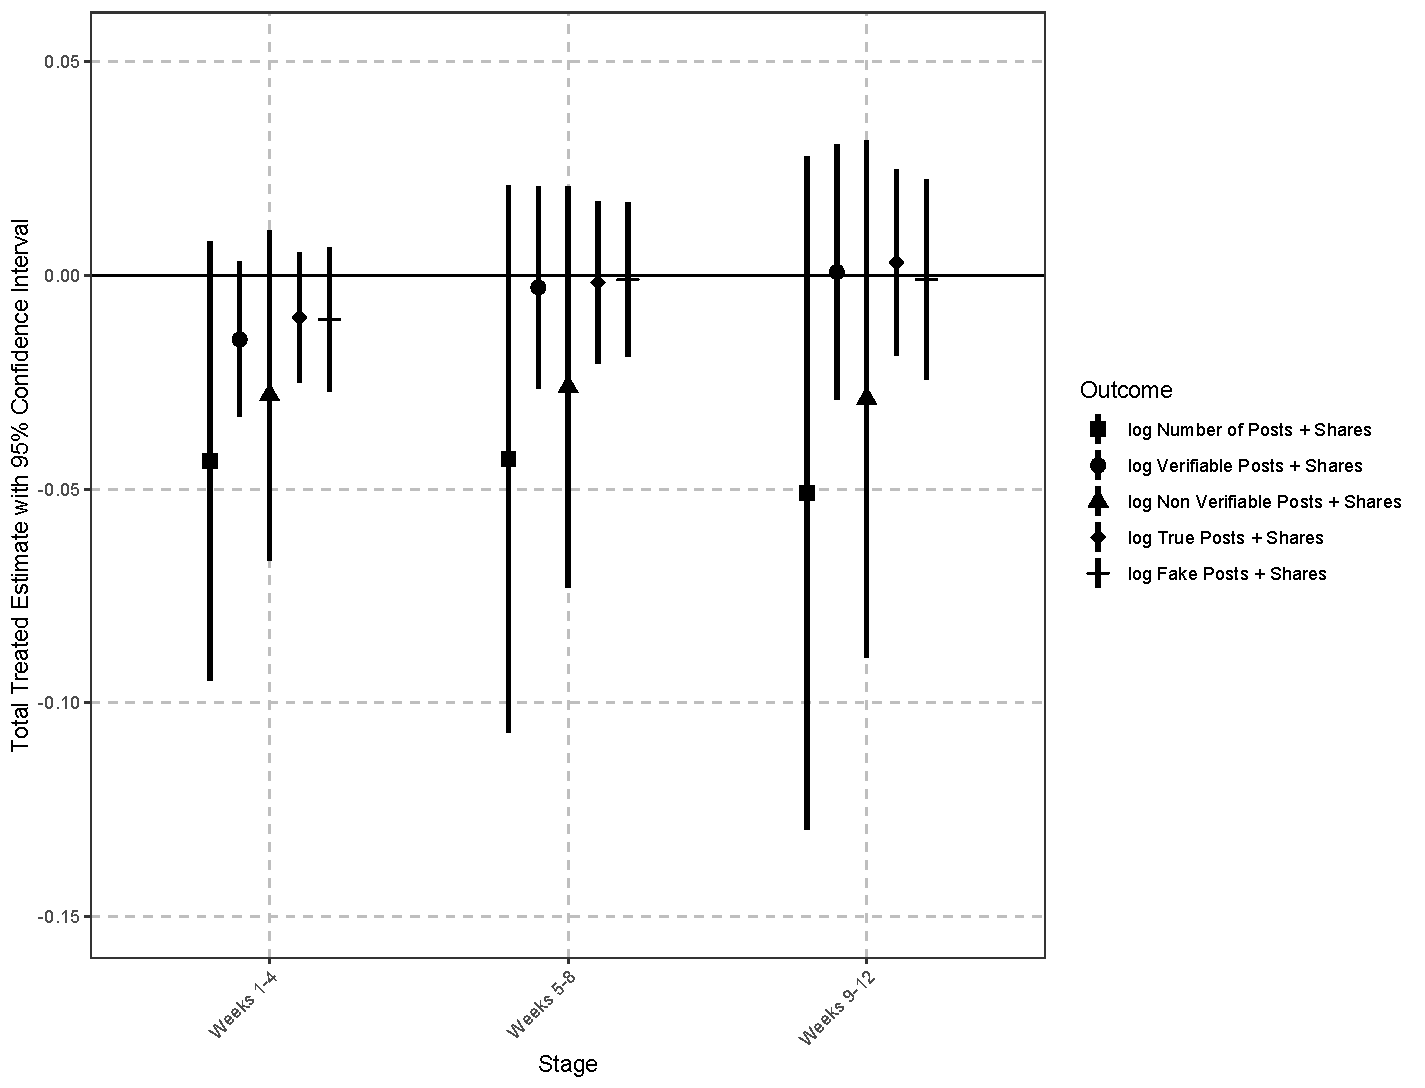
\includegraphics[width=\textwidth]{../results/replots/extensive_linear_90p_p5/log_extensive_verifiability_fes_normal_p90_p5_b1_1000perm.pdf}
    \label{fig:appendix_extensive_stage_b1}
    \floatfoot{\textit{Notes:} The figure reports the estimated effect of treatment for the Batch 1 extensive-margin sample separately for Weeks 1--4, Weeks 5--8, and Weeks 9--12. Whiskers denote permutation-based 95\% confidence intervals.}
\end{figure}

\begin{figure}[!htbp]
    \centering
    \caption{Extensive Outcomes: Stage-by-Stage Effects, Strong-Follower Sample, Batch 1}
    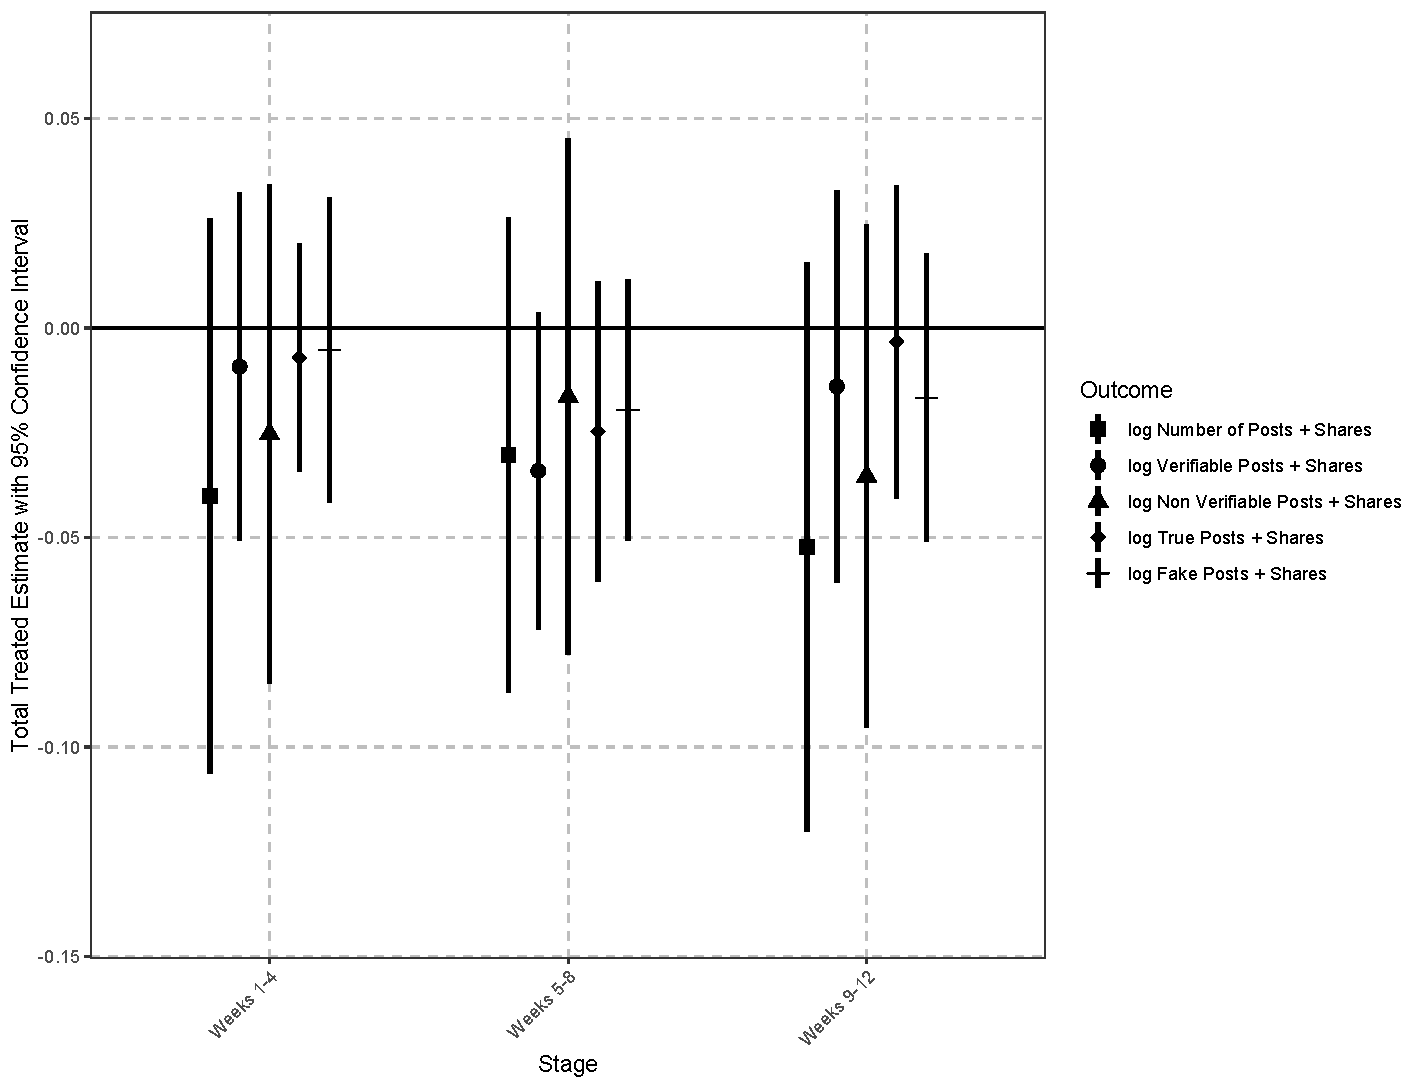
\includegraphics[width=\textwidth]{../results/replots/extensive_linear_90p_p5_strong/log_extensive_verifiability_fes_normal_p90_p5_strong_b1_1000perm.pdf}
    \label{fig:appendix_extensive_stage_strong_b1}
    \floatfoot{\textit{Notes:} The figure reports the estimated effect of treatment for the Batch 1 strong-follower sample separately for Weeks 1--4, Weeks 5--8, and Weeks 9--12. Whiskers denote permutation-based 95\% confidence intervals.}
\end{figure}

\begin{figure}[!htbp]
    \centering
    \caption{Intensive Outcomes: Stage-by-Stage Effects, Batch 1}
    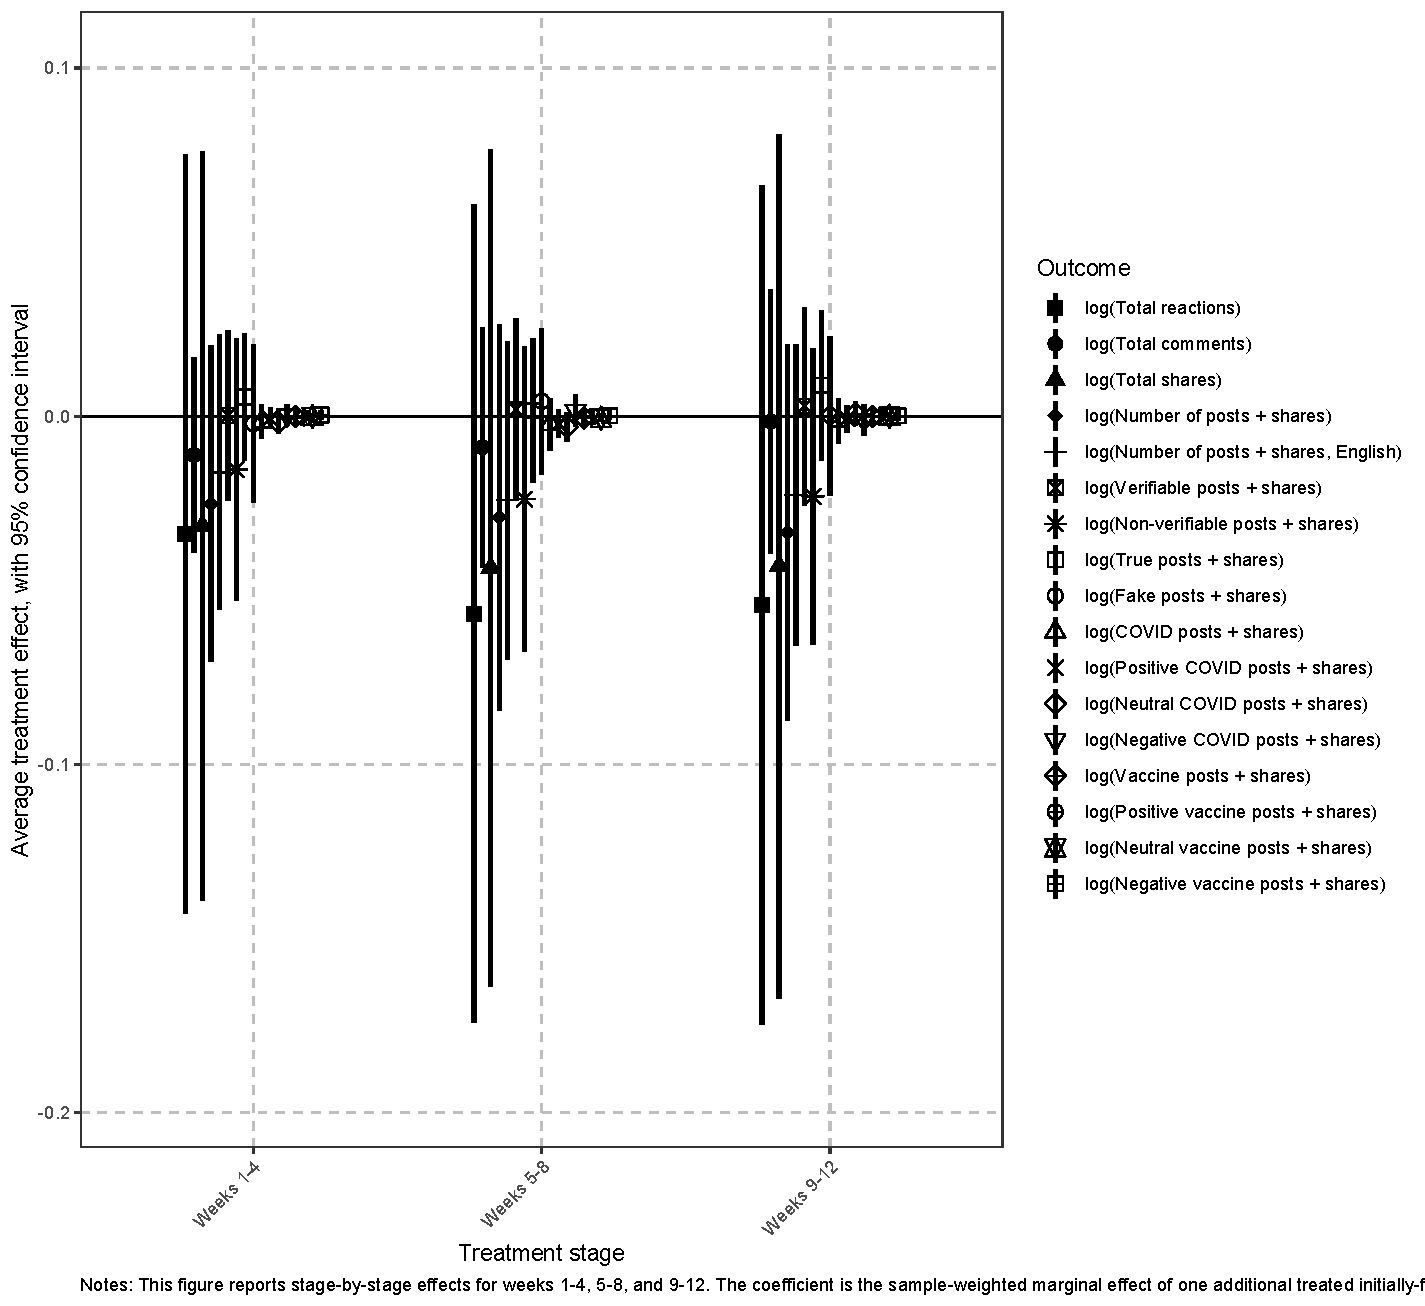
\includegraphics[width=\textwidth]{../results/replots/intensive_linear_95p_weighted/log_intensive_linear_95p_weighted_b1_1000perm.pdf}
    \label{fig:appendix_intensive_stage_b1}
    \floatfoot{\textit{Notes:} The figure reports the estimated effect of treatment for the Batch 1 intensive-margin sample separately for Weeks 1--4, Weeks 5--8, and Weeks 9--12. Whiskers denote permutation-based 95\% confidence intervals.}
\end{figure}

\subsection{Batch 1 Baseline Results}

\begin{figure}[!htbp]
    \centering
    \caption{Extensive Outcomes: Baseline Effects, Batch 1}
    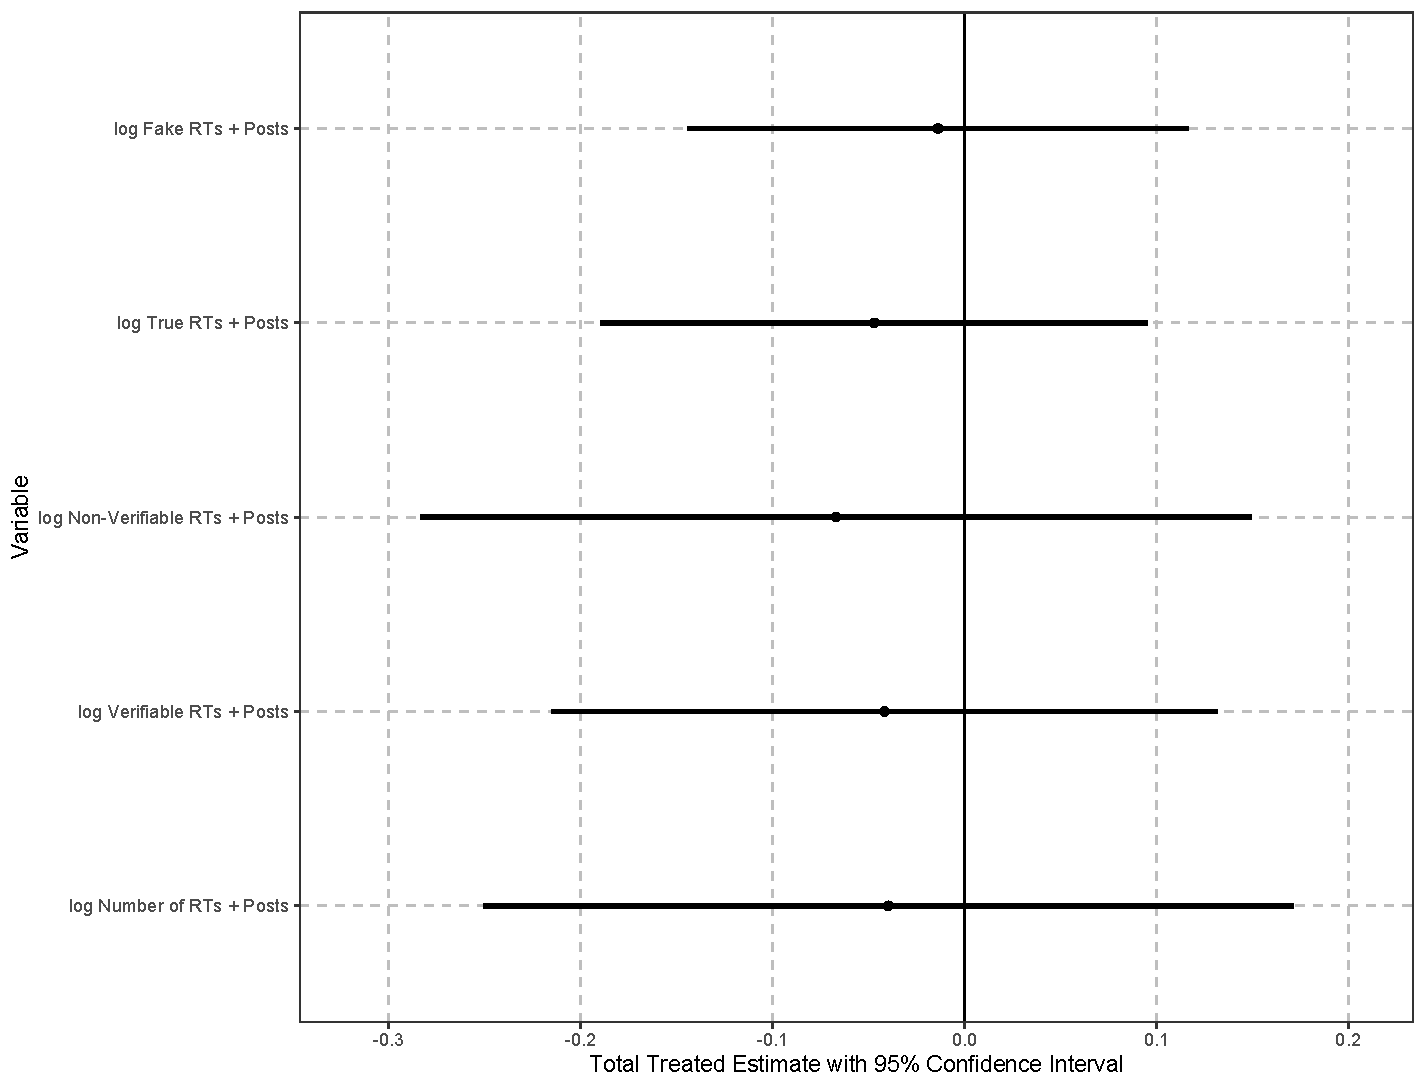
\includegraphics[width=\textwidth]{../results/replots/extensive/log_extensive_verifiability_noblockfes_p90_p0_b1_1000perm.pdf}
    \label{fig:appendix_extensive_baseline_b1}
    \floatfoot{\textit{Notes:} The figure reports the estimated treatment-control differences in baseline extensive outcomes for the Batch 1 sample. Whiskers denote permutation-based 95\% confidence intervals.}
\end{figure}

\begin{figure}[!htbp]
    \centering
    \caption{Extensive Outcomes: Baseline Effects, Strong-Follower Sample, Batch 1}
    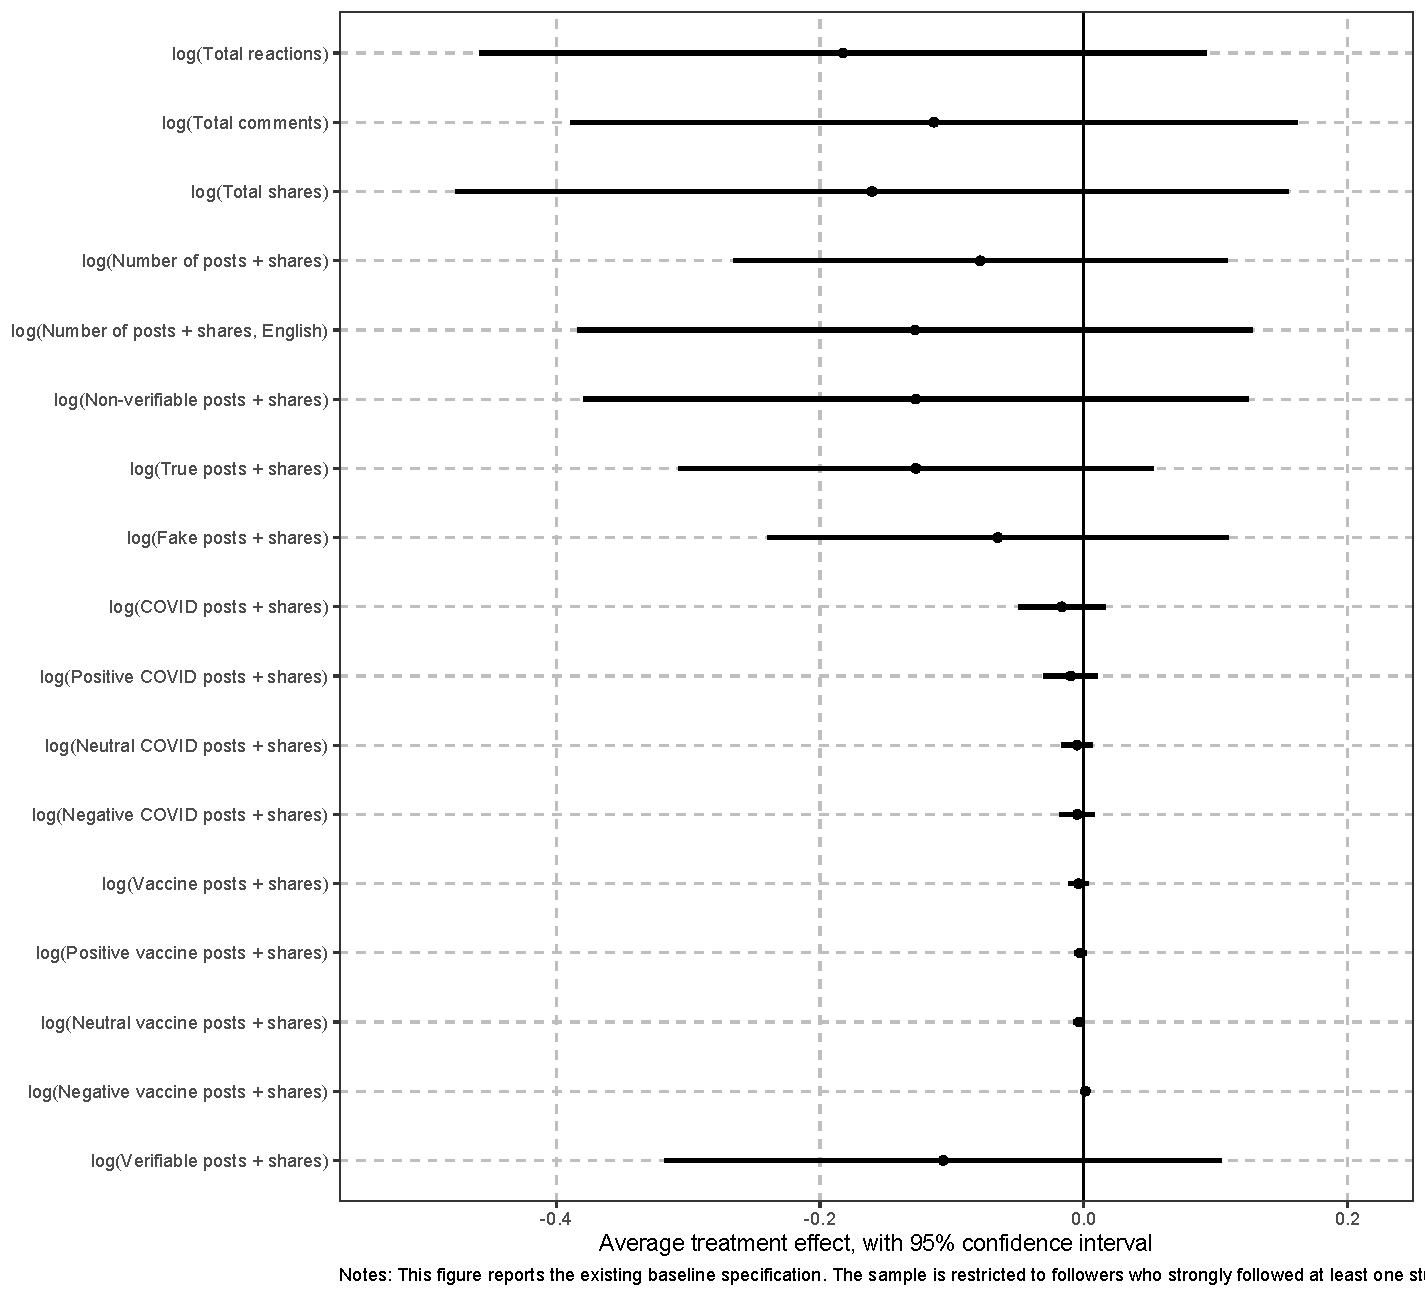
\includegraphics[width=\textwidth]{../results/replots/extensive_strong/log_extensive_verifiability_noblockfes_p90_p0_strong_b1_1000perm.pdf}
    \label{fig:appendix_extensive_baseline_strong_b1}
    \floatfoot{\textit{Notes:} The figure reports the estimated treatment-control differences in baseline extensive outcomes for the Batch 1 strong-follower sample. Whiskers denote permutation-based 95\% confidence intervals.}
\end{figure}

\begin{figure}[!htbp]
    \centering
    \caption{Intensive Outcomes: Baseline Effects, Batch 1}
    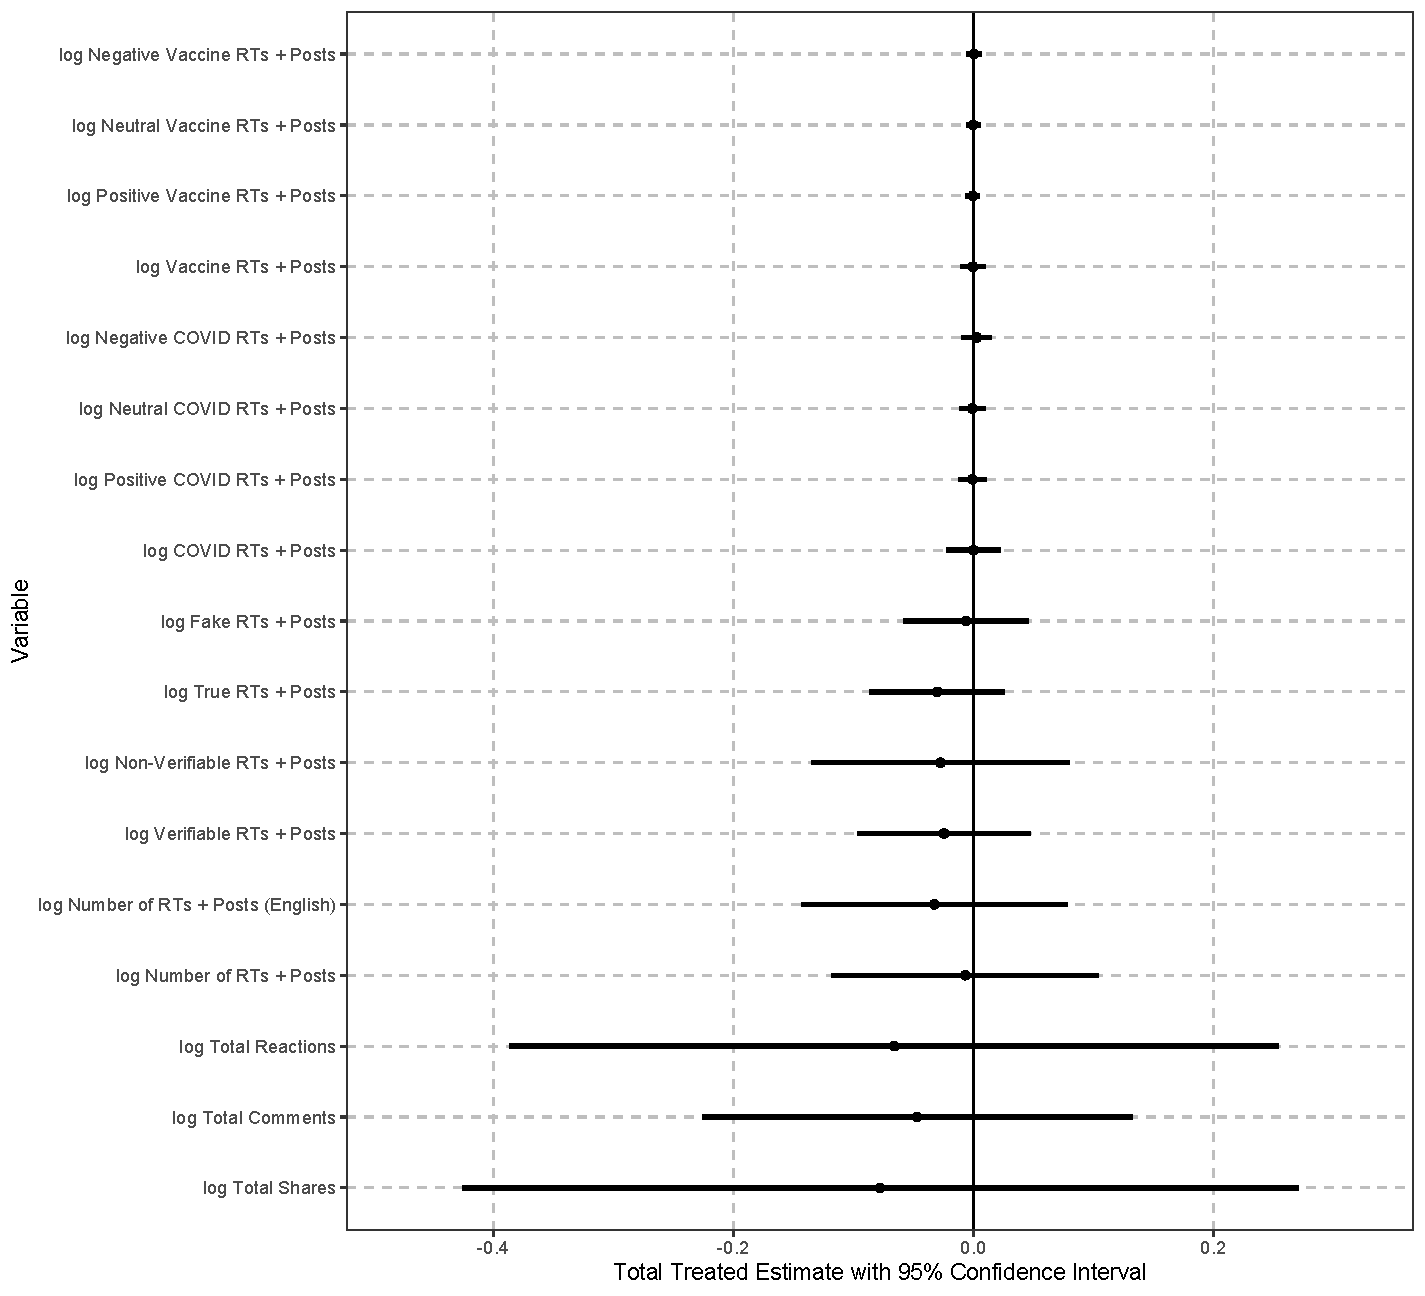
\includegraphics[width=\textwidth]{../results/replots/intensive_baseline_weighted/log_intensive_baseline_weighted_b1_1000perm.pdf}
    \label{fig:appendix_intensive_baseline_b1}
    \floatfoot{\textit{Notes:} The figure reports the estimated treatment-control differences in baseline intensive outcomes for the Batch 1 sample. Whiskers denote permutation-based 95\% confidence intervals.}
\end{figure}

\subsection{Aggregated Batch 2 and Both-Batch Results}

\begin{figure}[!htbp]
    \centering
    \caption{Extensive Outcomes: Aggregated Treatment-Period Effects, Batch 2}
    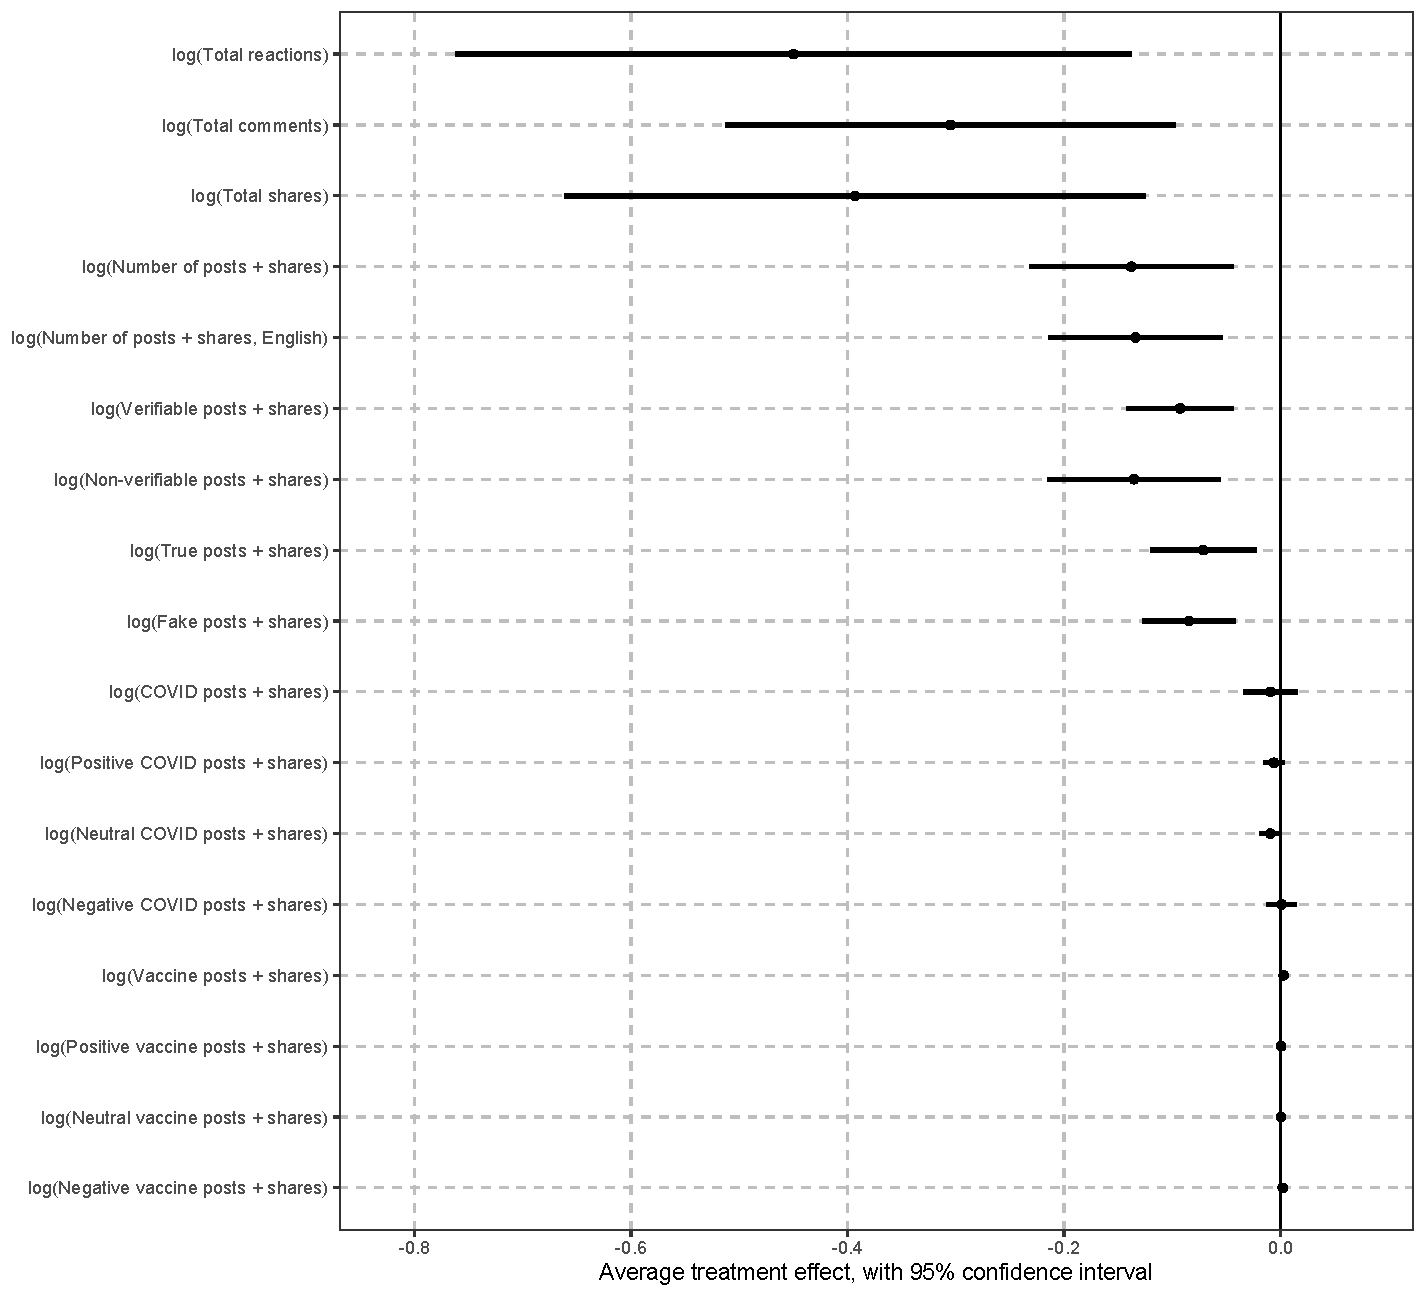
\includegraphics[width=\textwidth]{../results/replots/extensive_aggregate_batches/log_extensive_aggregate_batches_b2_1000perm.pdf}
    \label{fig:appendix_extensive_aggregate_b2}
    \floatfoot{\textit{Notes:} The figure reports the estimated effect of treatment for the Batch 2 extensive-margin sample after aggregating outcomes across Weeks 1--12. Whiskers denote permutation-based 95\% confidence intervals.}
\end{figure}

\begin{figure}[!htbp]
    \centering
    \caption{Extensive Outcomes: Aggregated Treatment-Period Effects, Both Batches}
    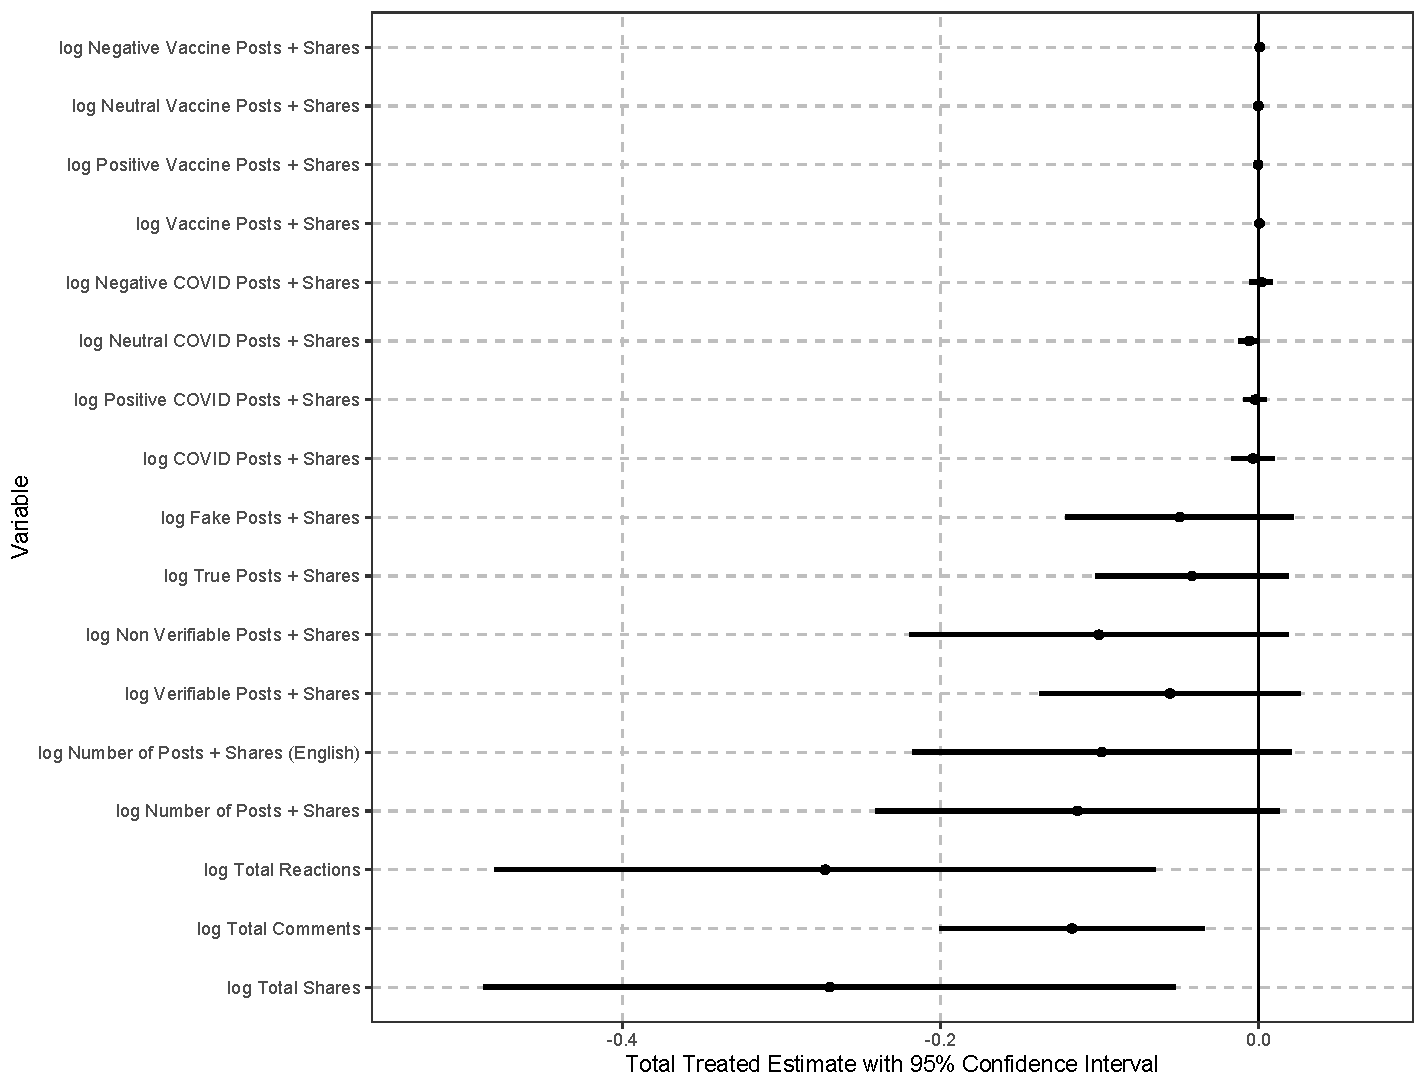
\includegraphics[width=\textwidth]{../results/replots/extensive_aggregate_batches/log_extensive_aggregate_batches_both_1000perm.pdf}
    \label{fig:appendix_extensive_aggregate_both}
    \floatfoot{\textit{Notes:} The figure reports the estimated effect of treatment for the pooled extensive-margin sample after aggregating outcomes across Weeks 1--12. Whiskers denote permutation-based 95\% confidence intervals.}
\end{figure}

\begin{figure}[!htbp]
    \centering
    \caption{Intensive Outcomes: Aggregated Treatment-Period Effects, Batch 2}
    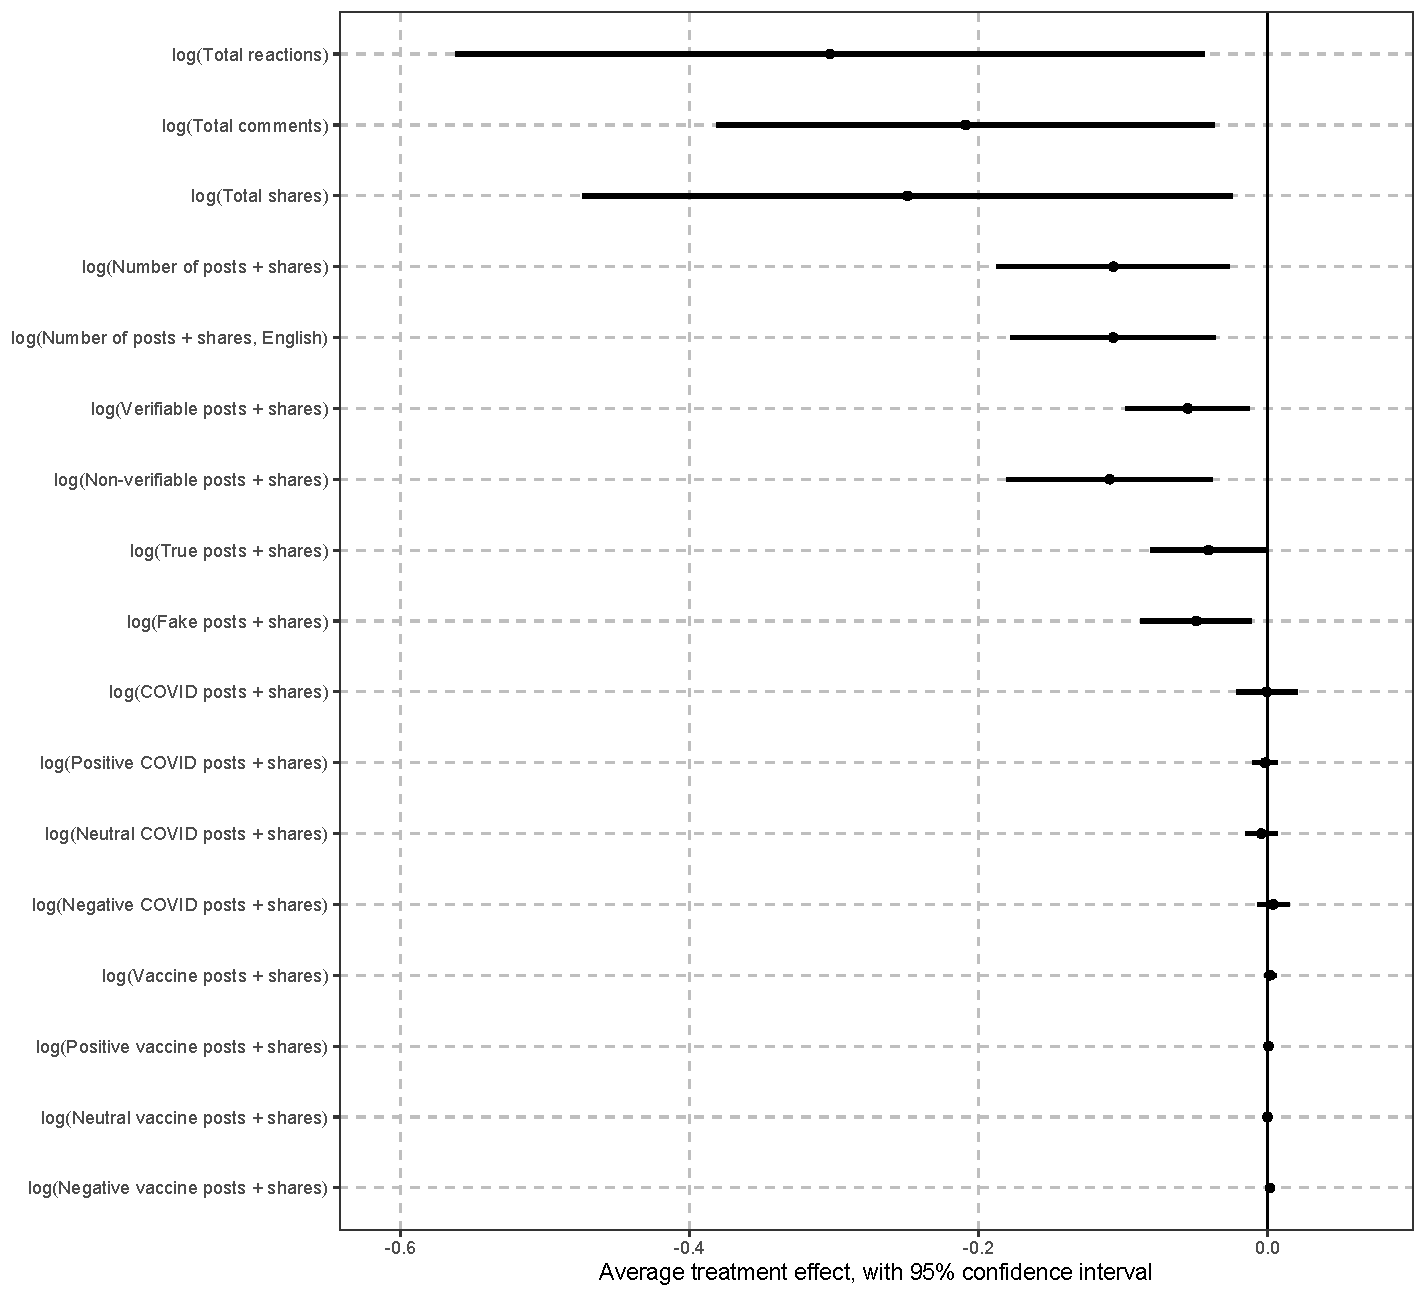
\includegraphics[width=\textwidth]{../results/replots/intensive_aggregate_batches/log_intensive_aggregate_batches_b2_1000perm.pdf}
    \label{fig:appendix_intensive_aggregate_b2}
    \floatfoot{\textit{Notes:} The figure reports the estimated effect of treatment for the Batch 2 intensive-margin sample after aggregating outcomes across Weeks 1--12. Whiskers denote permutation-based 95\% confidence intervals.}
\end{figure}

\begin{figure}[!htbp]
    \centering
    \caption{Intensive Outcomes: Aggregated Treatment-Period Effects, Both Batches}
    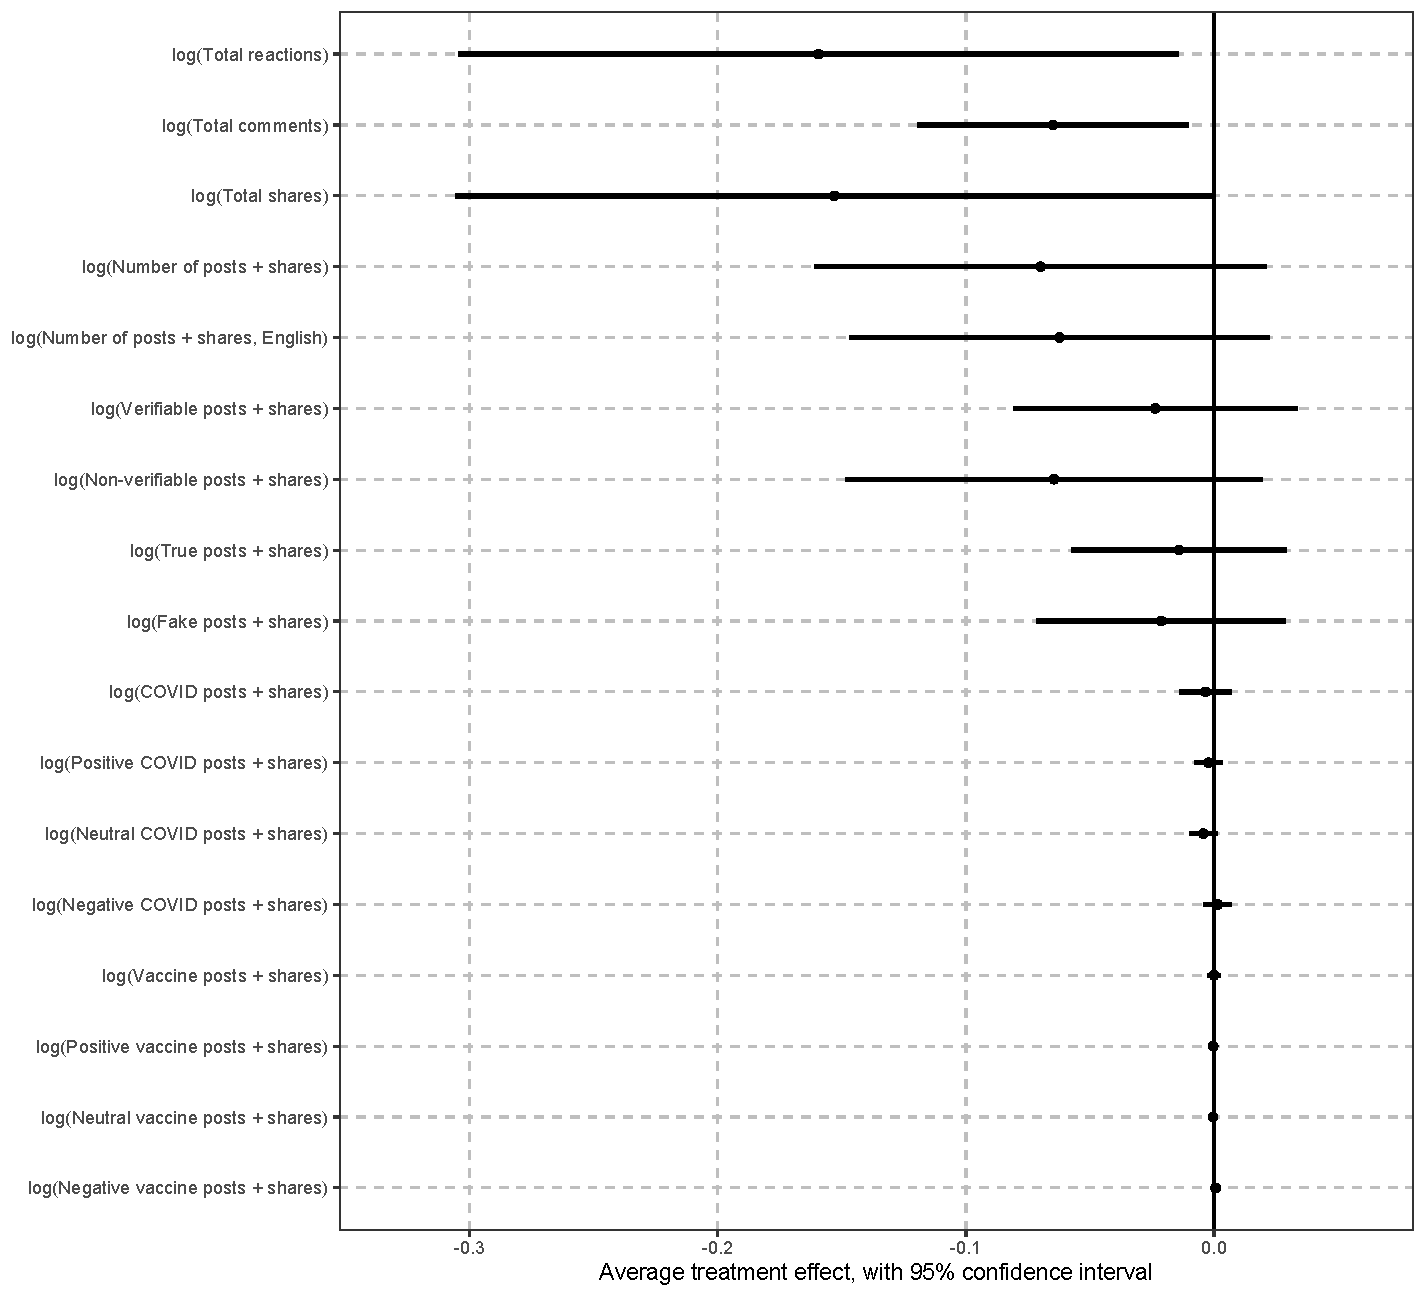
\includegraphics[width=\textwidth]{../results/replots/intensive_aggregate_batches/log_intensive_aggregate_batches_both_1000perm.pdf}
    \label{fig:appendix_intensive_aggregate_both}
    \floatfoot{\textit{Notes:} The figure reports the estimated effect of treatment for the pooled intensive-margin sample after aggregating outcomes across Weeks 1--12. Whiskers denote permutation-based 95\% confidence intervals.}
\end{figure}

\subsection{Remaining Stage-by-Stage Results}

\begin{figure}[!htbp]
    \centering
    \caption{Extensive Outcomes: Stage-by-Stage Effects, Batch 2}
    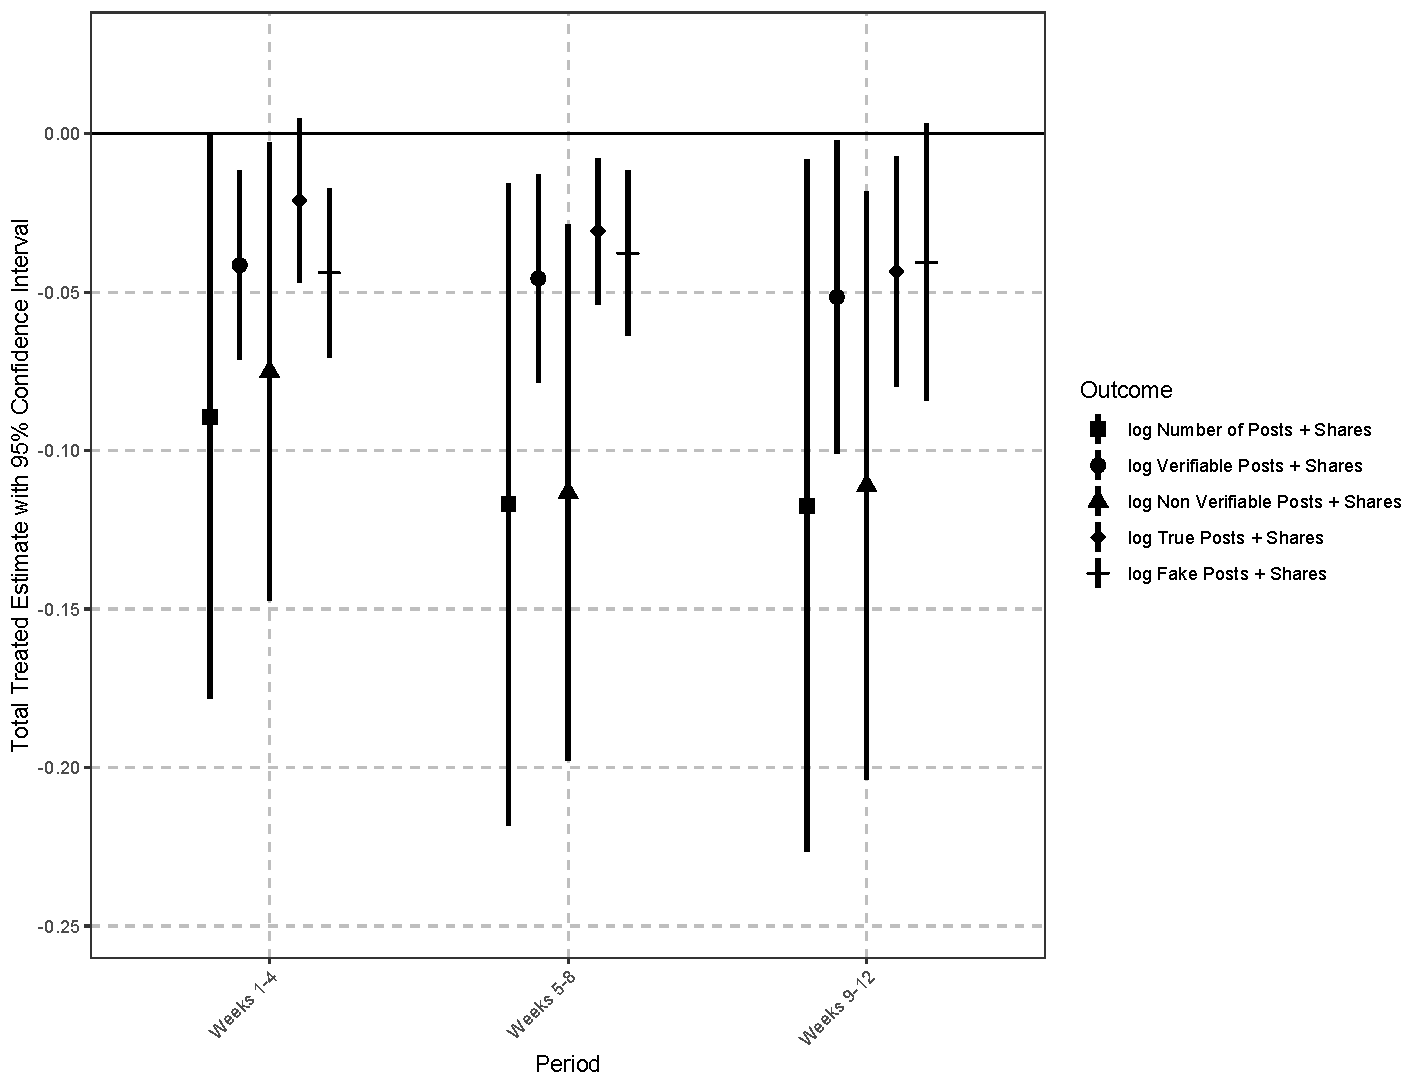
\includegraphics[width=\textwidth]{../results/replots/extensive_linear_90p_p5/log_extensive_verifiability_fes_normal_p90_p5_b2_1000perm.pdf}
    \label{fig:appendix_extensive_stage_b2}
    \floatfoot{\textit{Notes:} The figure reports the estimated effect of treatment for the Batch 2 extensive-margin sample separately for Weeks 1--4, Weeks 5--8, and Weeks 9--12. Whiskers denote permutation-based 95\% confidence intervals.}
\end{figure}

\begin{figure}[!htbp]
    \centering
    \caption{Extensive Outcomes: Stage-by-Stage Effects, Strong-Follower Sample, Batch 2}
    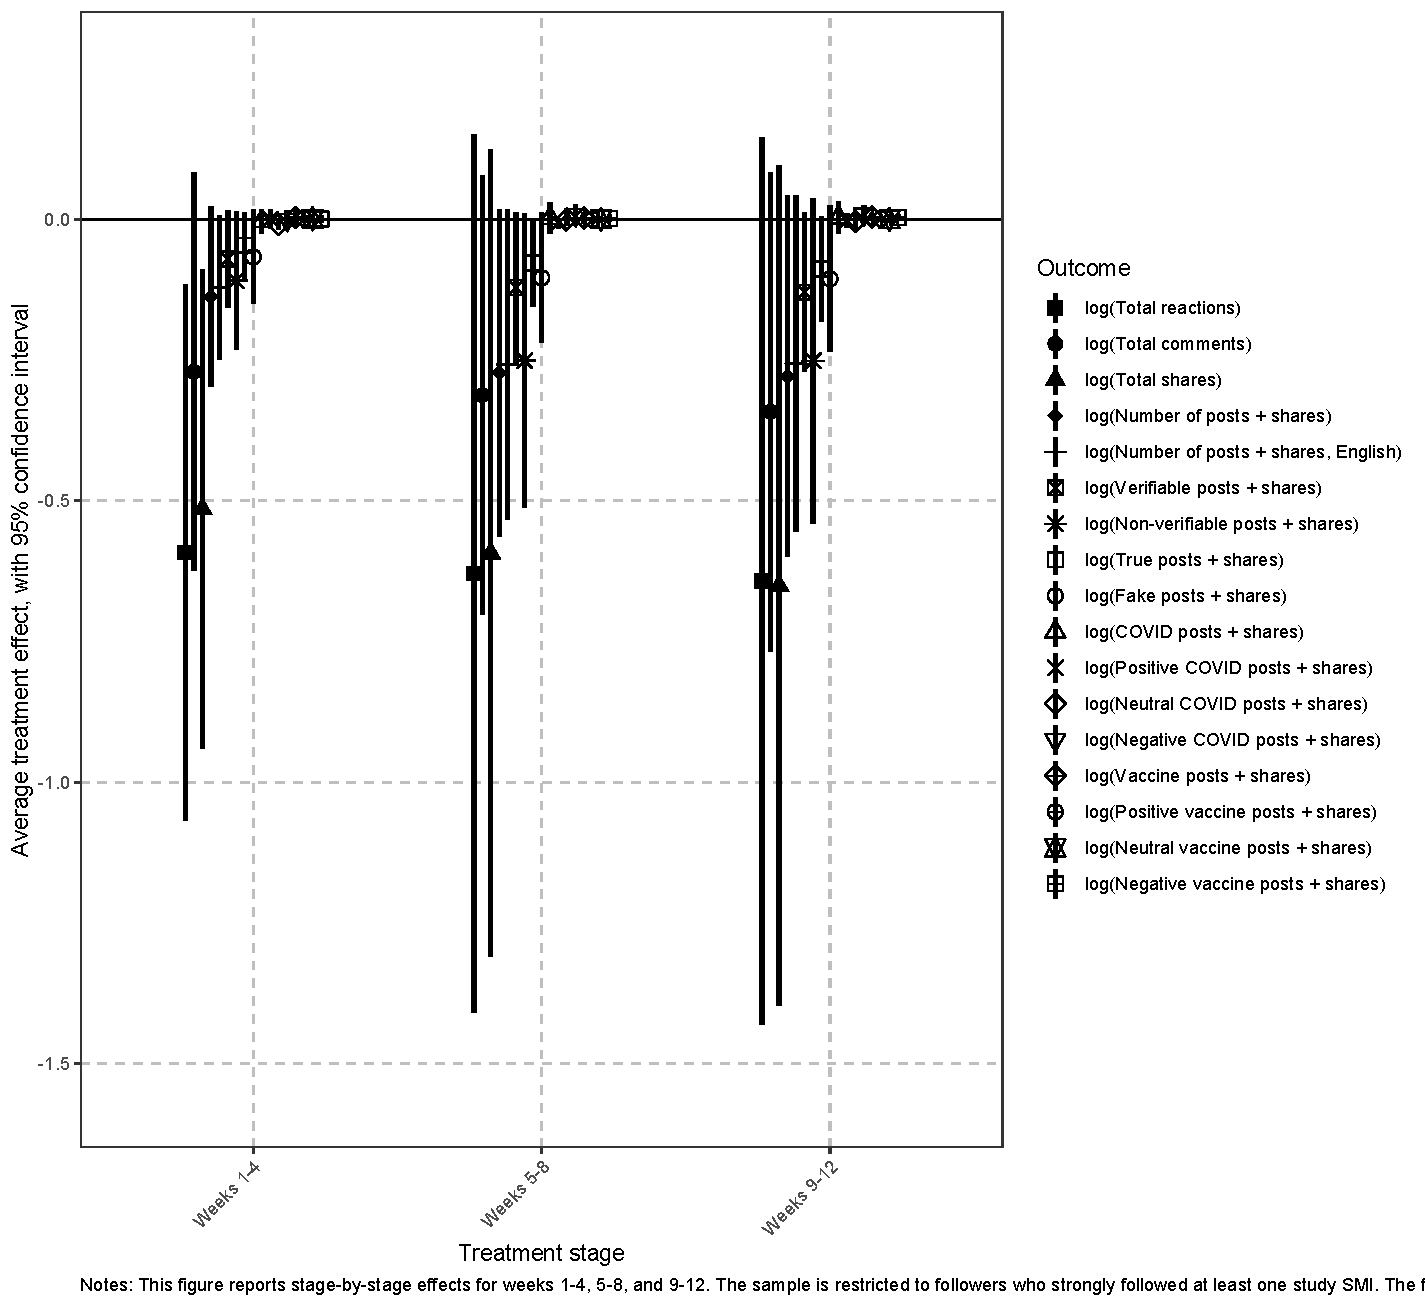
\includegraphics[width=\textwidth]{../results/replots/extensive_linear_90p_p5_strong/log_extensive_verifiability_fes_normal_p90_p5_strong_b2_1000perm.pdf}
    \label{fig:appendix_extensive_stage_strong_b2}
    \floatfoot{\textit{Notes:} The figure reports the estimated effect of treatment for the Batch 2 strong-follower sample separately for Weeks 1--4, Weeks 5--8, and Weeks 9--12. Whiskers denote permutation-based 95\% confidence intervals.}
\end{figure}

\begin{figure}[!htbp]
    \centering
    \caption{Intensive Outcomes: Stage-by-Stage Effects, Batch 2}
    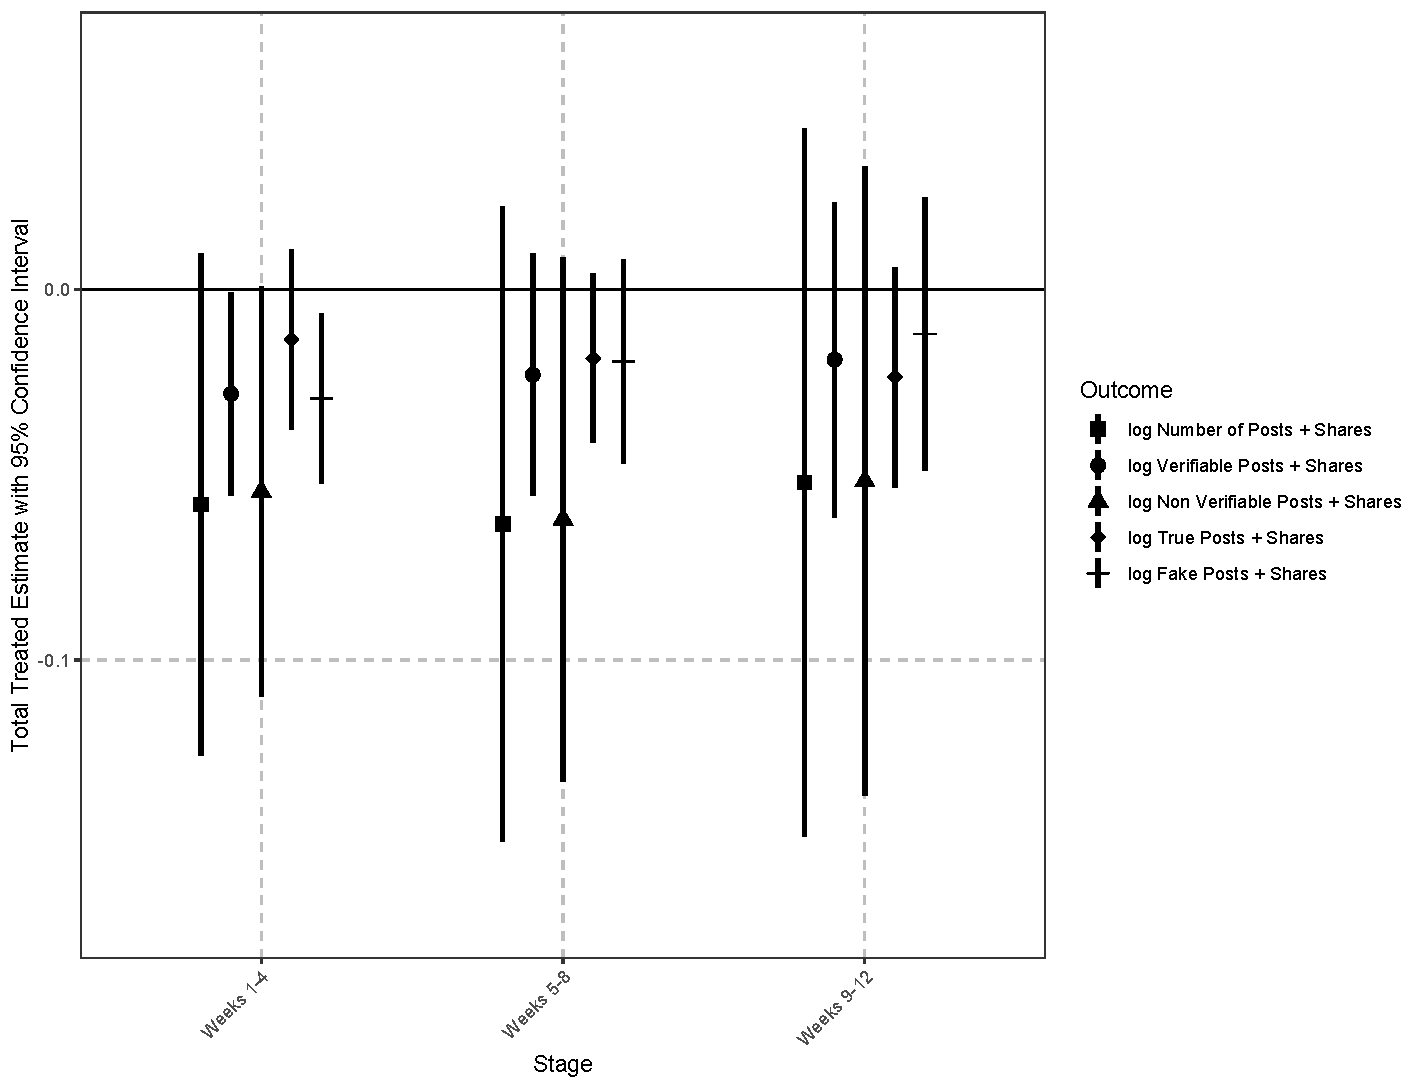
\includegraphics[width=\textwidth]{../results/replots/intensive_linear_95p_weighted/log_intensive_linear_95p_weighted_b2_1000perm.pdf}
    \label{fig:appendix_intensive_stage_b2}
    \floatfoot{\textit{Notes:} The figure reports the estimated effect of treatment for the Batch 2 intensive-margin sample separately for Weeks 1--4, Weeks 5--8, and Weeks 9--12. Whiskers denote permutation-based 95\% confidence intervals.}
\end{figure}

\begin{figure}[!htbp]
    \centering
    \caption{Extensive Outcomes: Stage-by-Stage Effects, Both Batches}
    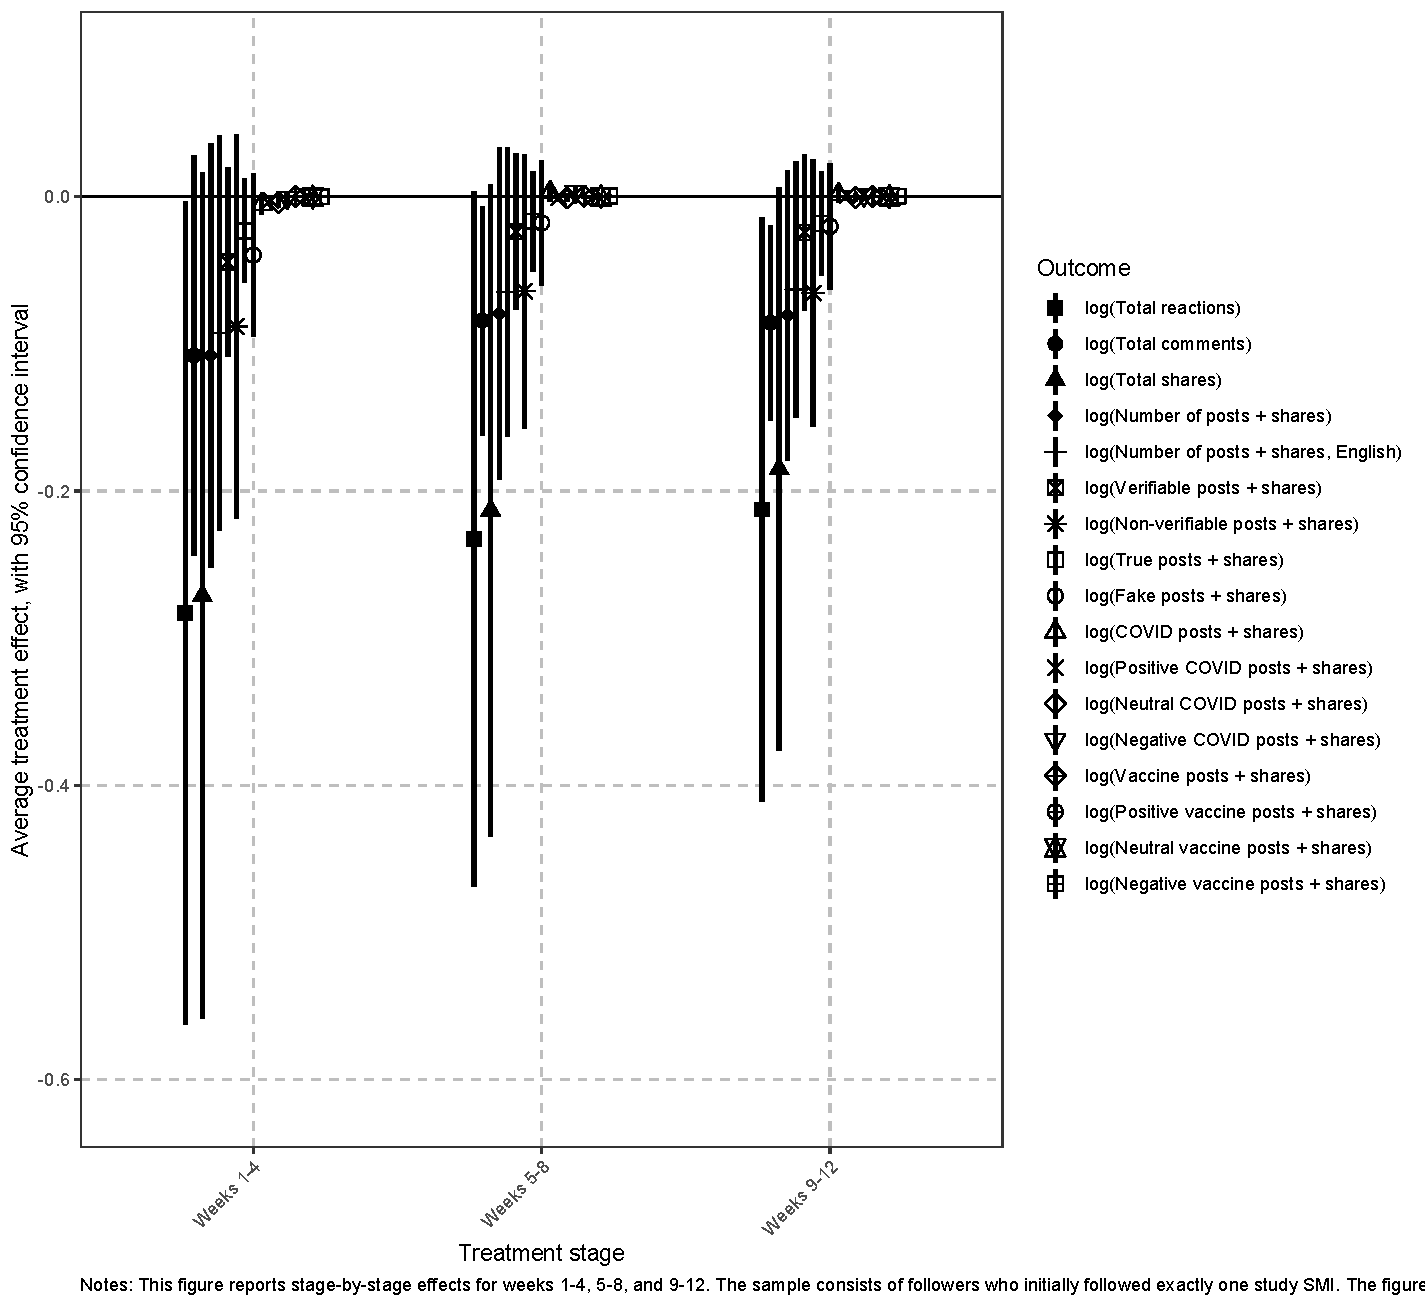
\includegraphics[width=\textwidth]{../results/replots/extensive_linear_90p_p5/log_extensive_verifiability_fes_normal_p90_p5_both_1000perm.pdf}
    \label{fig:appendix_extensive_stage_both}
    \floatfoot{\textit{Notes:} The figure reports the estimated effect of treatment for the pooled extensive-margin sample separately for Weeks 1--4, Weeks 5--8, and Weeks 9--12. Whiskers denote permutation-based 95\% confidence intervals.}
\end{figure}

\begin{figure}[!htbp]
    \centering
    \caption{Extensive Outcomes: Stage-by-Stage Effects, Strong-Follower Sample, Both Batches}
    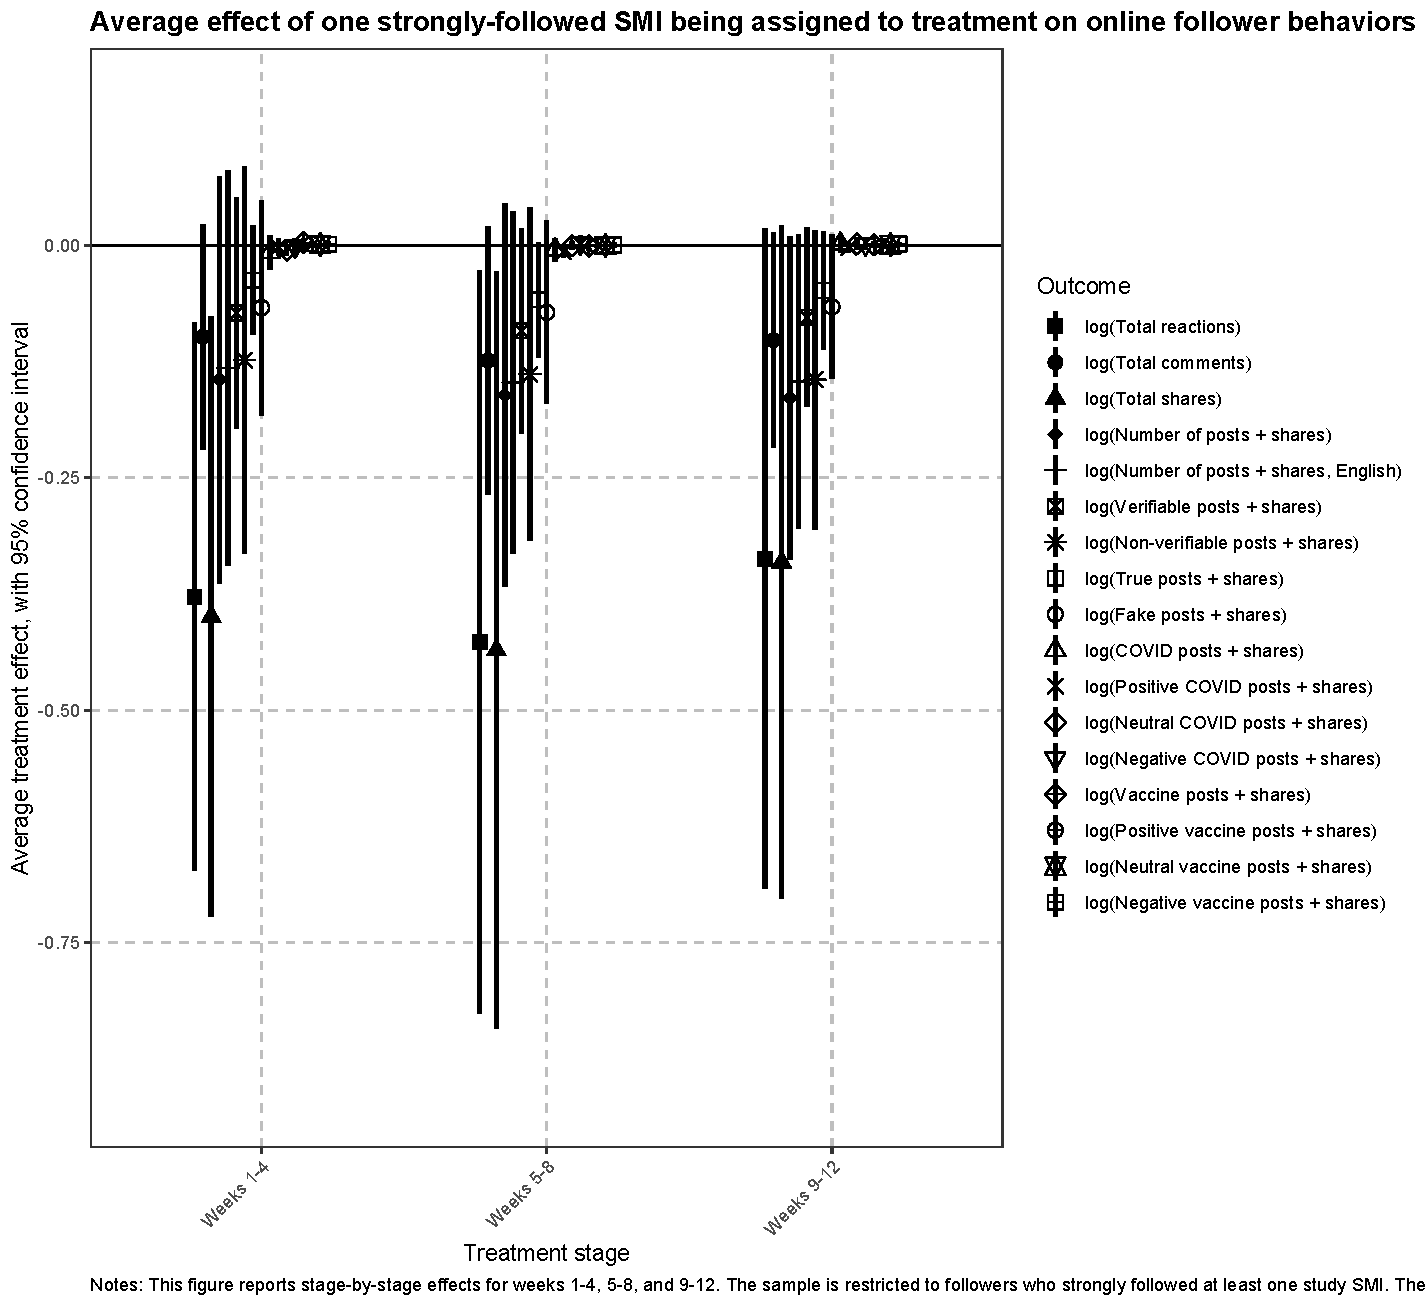
\includegraphics[width=\textwidth]{../results/replots/extensive_linear_90p_p5_strong/log_extensive_verifiability_fes_normal_p90_p5_strong_both_1000perm.pdf}
    \label{fig:appendix_extensive_stage_strong_both}
    \floatfoot{\textit{Notes:} The figure reports the estimated effect of treatment for the pooled strong-follower sample separately for Weeks 1--4, Weeks 5--8, and Weeks 9--12. Whiskers denote permutation-based 95\% confidence intervals.}
\end{figure}

\begin{figure}[!htbp]
    \centering
    \caption{Intensive Outcomes: Stage-by-Stage Effects, Both Batches}
    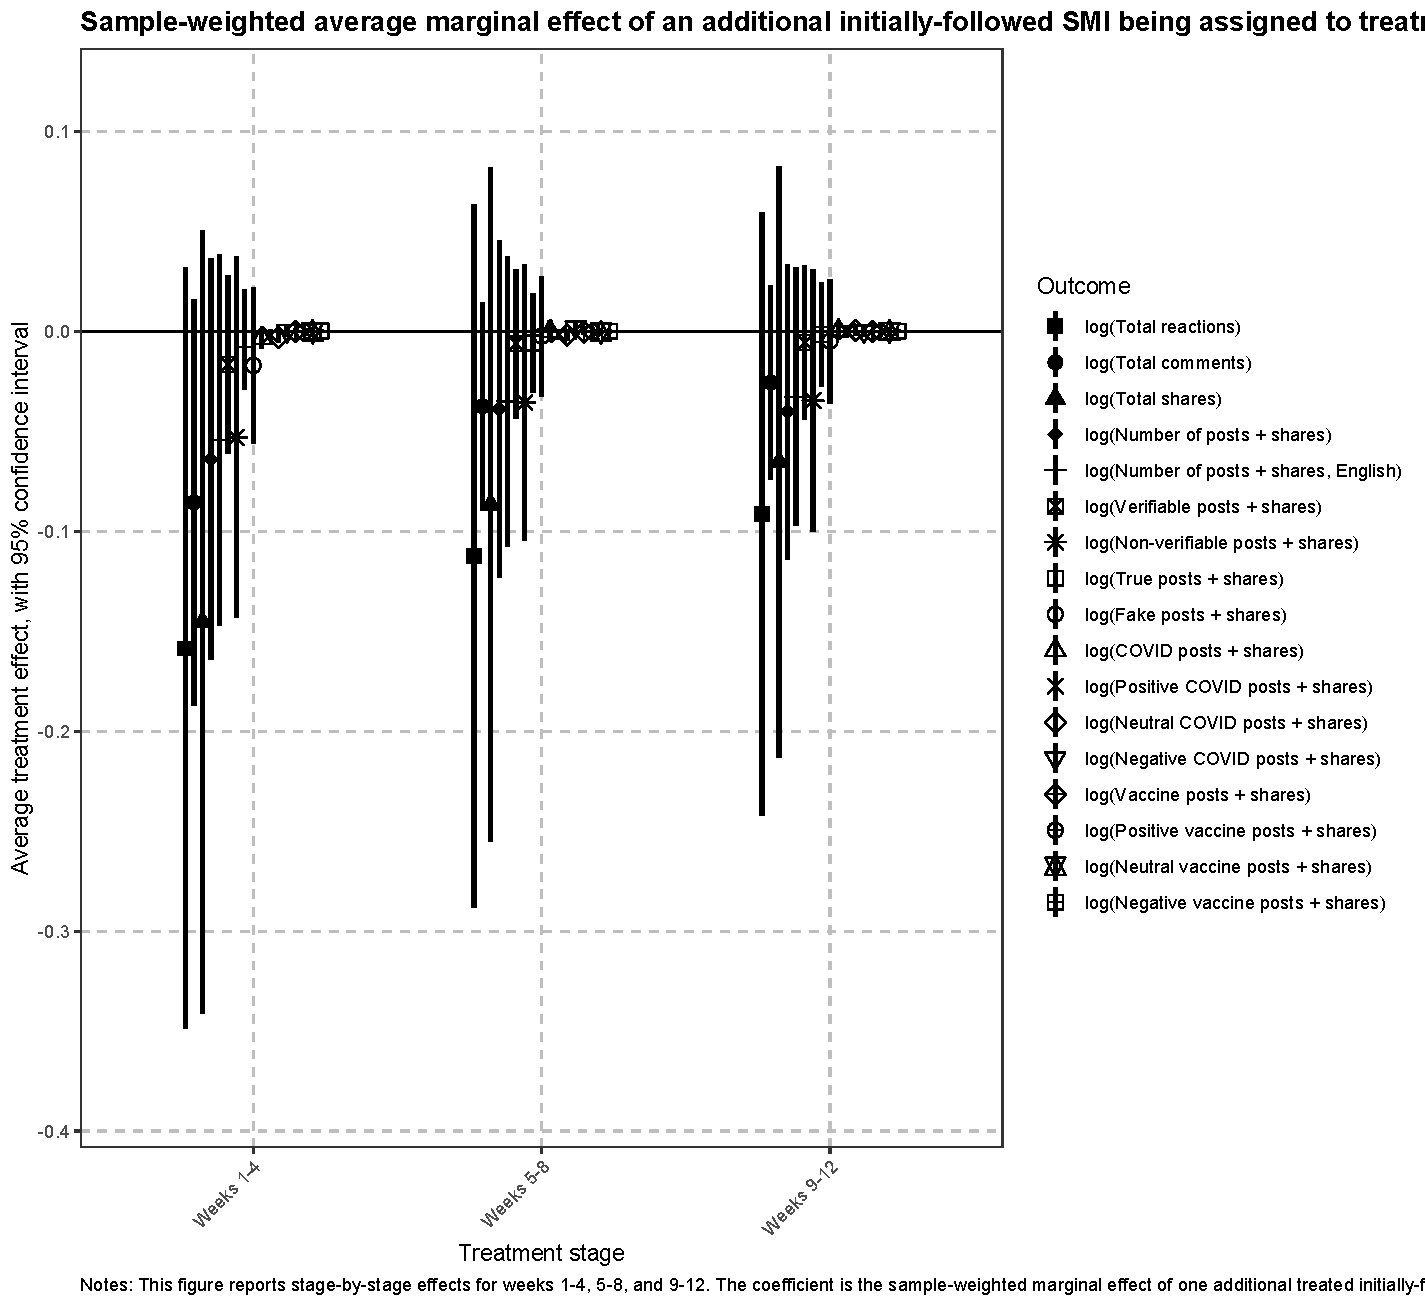
\includegraphics[width=\textwidth]{../results/replots/intensive_linear_95p_weighted/log_intensive_linear_95p_weighted_both_1000perm.pdf}
    \label{fig:appendix_intensive_stage_both}
    \floatfoot{\textit{Notes:} The figure reports the estimated effect of treatment for the pooled intensive-margin sample separately for Weeks 1--4, Weeks 5--8, and Weeks 9--12. Whiskers denote permutation-based 95\% confidence intervals.}
\end{figure}
